It is essential to any living species to recognise others in their community. Evolution has allowed animals to develop many methods, how to identify fellow members. Different species use various senses to do so. Smell, vision or hearing are the most common ones. However, humankind relies mostly on their vision. We did not develop strong perception of smell or other senses, that we can utilise on purpose or over longer distances. Therefore we mostly use our vision.

Moreover our species developed a habit to cover ourselves in clothes, which left only certain parts of our body exposed. Usually that's head and hands. And since receptors for most of our senses are placed on head, we are required to have it exposed to be able to orient in surroundings. This makes the frontal part of our head, a face, a great candidate for identifying others\,\cite{history}. We can recognise many nuances of different elements on the face. Shape of eyes, nose or mouth, colour of our eyes\dots That's just a subset of all the available features we use.

In this era of computers and information technologies, mankind tend to use what we know and offload our skills and capabilities to artificial intelligence. We hope to sharpen and enhance our senses; obtain more knowledge or widen our possibilities. As an example, which is more deeply elaborated in this thesis, we are trying to "teach" machines to recognise faces in the same way as we do. And there are various reasons to do so.

\section{Motivation}
Facial recognition in computer science is used in many different ways. Some use cases require people to be recognised for personal or company security purposes, for surveillance or just for our convenience.

Automating security countermeasures is a huge driving factor. It allows us to devote our time to other activities then watching over our belongings. It ensures our privacy and well being of the community. Let's list some basic use cases:

\begin{itemize}
    \item \textbf{Personal security}: unlocking a smartphone or laptop, etc.
    \item \textbf{Enterprise security and state defence}: access control, customs and border control, etc.
    \item \textbf{Surveillance}: Outlaws identification in public places, riot control, etc.
\end{itemize}

Furthermore, automated recognition of people's faces and their identification can facilitate many other processes for our convenience. That usually means it can save us time and provide a better service. These use cases spans from face and smile detection on when focusing and timing a camera shot to automated tagging of individual's friend on social media networks.

\section{Justification}

As in any other field in computer science, there is an ongoing race to provide better service in facial recognition. There are multiple aspects used as a metric to define better solution and this varies for each use case. Once, it is essential to provide the best performing software, for automated recognition, in places where limited computational power is available. Other time, it is rather about precision and time required to recognise a face. Outrunning other solutions means better service and inventing new technologies along the way unlocks better understanding on our own thinking process. In this thesis the existing solutions will be elaborated in detail as well as principles used to achieve such results.

There are also different approaches used to create and design such solutions. Sometimes a naive approach is used, other times the implementation leverages different aspects of Artificial Intelligence, especially Neural Networks.

The aim of this thesis is to construct a very own solution to this problem, relying strictly on Neural Networks. Each part of the problem is explained, while only the later one is the crucial and key deliverable for this thesis. Therefore only the actual facial recognition over already located faces is implemented. Comparison with existing solutions is offered as a part of the Available solutions chapter\,\ref{chapter:solutions}, later in this thesis.

\section{Decomposition}

To recognise a human face in a picture or video is a fairly complex problem. Therefore it is usually divided into smaller sub-tasks, which are easier to comprehend and solve. Firstly, it is required to understand the input data. This understanding provides means to fundamentally divide the problem into easily solvable sub-tasks. Let's define and describe what are the expectations and demands on the input, so we can assess plausible approaches and later understand each subtask as a separate problem. Then we can assume and thoroughly elaborate the desired outputs.

\subsection{In-the-wild pictures}

As wide as the use cases, the variety of input data is vast. Some cases depends on frontal pictures of faces, some accents the so-called \textit{in-the-wild} aspect. This is a term specifically used for pictures captured without cooperation of the subject. A person on the picture is usually captured from an angle, lacking eye contact and staged emotion, etc. This thesis aims to cover a topic of facial recognition over CCTV data. However it can be said that any in-the-wild pictures are suitable for this implementation. The sufficient resolution and recognizability is the most important feature and requirement on the input data. The model has to be able to find a face on the picture. Therefore even it the model would rely solely on CCTV data, the data feed has to provide enough detail of the person's face.

\begin{figure}[ht]
    \centering
    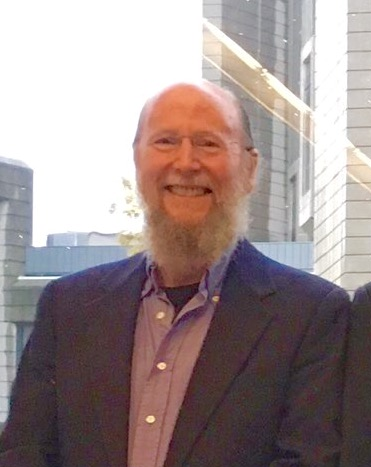
\includegraphics[height=15em]{obrazky-figures/richard_sutton.jpg}
    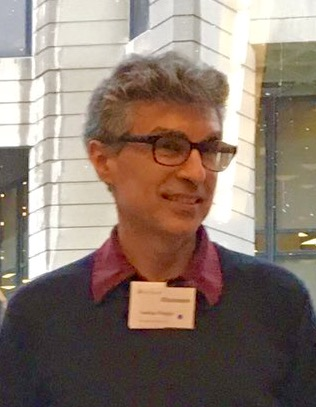
\includegraphics[height=15em]{obrazky-figures/yoshua_bengio.jpg}
    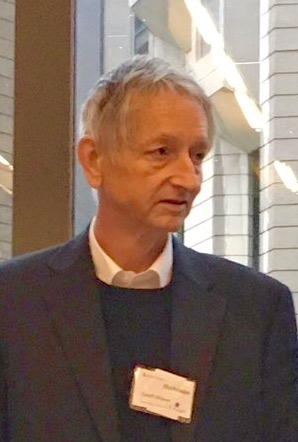
\includegraphics[height=15em]{obrazky-figures/geoffrey_hinton.jpg}
    \caption[Example of pictures in{-}the{-}wild]{Example of pictures in{-}the{-}wild. From left: Richard Sutton, Yoshua Bengio, Geoffrey Hinton. \textit{Source: Steve Jurvetson (CC BY 2.0\,\footnotemark)}}
\end{figure}

CCTV as a source of the input data has some crucial advantages for real world scenarios over any random pictures in-the-wild. Usually CCTV produces feeds, therefore the subject of recognition is captured on many frames of a video recording. That means, the model can be provided by many images of the same face and if properly configured and trained, it can leverage this aspect.

In our scenario, this data has to be simplified and preprocessed since our main interest lays in the field of identity mapping for each face. Therefore instead of a full, legit CCTV footage, we will mainly work with already located and isolated, face centered images. More detail elaboration of the input data can be found in chapter \ref{chapter:implementation}.

\subsection{Recognition and identification}
\footnotetext{\url{https://creativecommons.org/licenses/by/2.0/deed.en}}

Imagine an individual captured on a CCTV footage. To identify a person by face, we have to naturally focus the model on the face. Therefore the first step would be to detect where and if the picture captures a face. When such region is found, it is essential to detect all the facial features the models is trained to focus. Not always all features are available (the face can be partially covered, captured from an angle etc.)\,--\,the model has to adapt to such situation. Based on features detected, the model creates an normalised estimation of facial features. This normalised template should represent a frontal scan of facial features of the individual's face. When the model has access to multiple images of the face, it can produce multiple templates and combine them into one unique normalised master template, unique to the person.

\subsection{Output information}

Last but not least, let's define what is expected to be found in such pictures. A facial identification model aims to come up with a unique vector (face template) for each person. Unique in a sense of minimising inter-dimensionality and maximising intra-dimensionality. That means the vector extracted from a picture is similar to all other vectors for the same person, as much as possible. It is also the most different to vector assigned to other people. Naturally each picture of the same person can result into slightly different template. However this sample specific output vector is expected to be nearly identical to a summarised template for the person. This summarised template is a result of combining many output vectors for the same individual. In this thesis we will elaborate more simplistic approach which will result into comparable results, yet more convenient and better consumable output.
